\textbf{COLUNI 2025 -- Questão 32}\par\medskip Observe a imagem a seguir que retrata parte da área urbana do município de Viçosa-MG.

\begin{center}
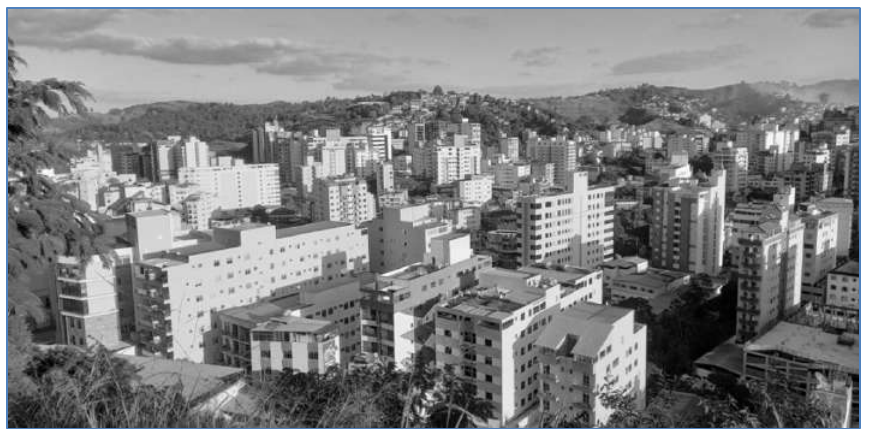
\includegraphics[width=0.75\linewidth]{static/simulados/coluni/figuras/2025/questao-32/figura-1.png}\\
Fonte: Léo Tiradentes (Agosto 2023).
\end{center}

Localizada na Zona da Mata Mineira, onde predominam as formas denominadas “mares de morros”, o município de Viçosa possui população aproximada de 80.000 habitantes - sendo mais de 90\% residente em áreas urbanas - e apresenta densidade demográfica de $255\,\text{hab}/\text{km}^2$. Segundo o IBGE (2023), Viçosa é uma das cidades mais verticalizadas do Brasil.

Sobre o fenômeno da verticalização urbana, é CORRETO afirmar que:
\begin{enumerate}
\item o território brasileiro vem passando por um crescimento urbano, fruto da concentração populacional, principalmente nas pequenas cidades, onde a migração rural urbana intensificou o processo de verticalização.
\item a verticalização é um fenômeno urbano resultado de um acelerado crescimento vertical, principalmente no núcleo central das cidades, podendo ocasionar problemas sociais e ambientais, caso não exista uma política pública de planejamento urbano.
\item a presença de um relevo com muitas serras e morros impede o crescimento das cidades para as áreas mais periféricas, estimulando a verticalização da área central, aumentando a densidade demográfica e reduzindo a qualidade de vida.
\item a verticalização pode apresentar motivos e características diversas conforme a localidade; em Viçosa o fenômeno se deve a uma intensa especulação imobiliária, associada à economia cafeeira para a qual são destinados os melhores investimentos.
\end{enumerate}
